\chapter{Implementation}
\label{chapter:implementation}

\begin{itemize}
  \item intro
  \item Vi lager en liten prototype = ``proof of concept'' -> et begrep vi m\aa~bruke =)
  \item VarRefs m\aa~sendes oppover fra child nodes (ref til tainting deps)
  \item Optimalisering: child nodes vet om de er atomiske/singleton eller ikke
\end{itemize}

\begin{itemize}
  \item Bruk av parseren (den som er generert av antlr osv), XQFTTree-klassen,
  evt. UML
  \item Interfacing av parseren mot oversetteren v\aa r (som oversetter til
  relalg) og UML
  \item Bygging av relasjonsalgebra-tre, UML av operatorklassene
  \item Implementering av visitors
  \item Scoping og symtab (nok en gang..)
  \item hvordan metadata som varrefs og singletonindikering blir sendt oppover
  (Metadata)
  \item Implementering av ``tainting dependencies''
  \item Dataflyt ()
  \item Visible external API
  \item Interface til systemet p\aa~ kommandolinjen
  \item Optimaliseringer, om noen? 
\end{itemize}

\section{Prerequisites}
This proof of concept was implemented in Java 5.0, using regular object
oriented techniques, and is licensed under a liberal BSD license. Instructions
for compilation and installation can be found in TODO: appendix.

\section{Overall system description}
A simplified class diagram describing the essentials of the system is shown in
figure \ref{fig:impl:sys:uml_complete}.

\begin{figure}[!htp]
\begin{center}
  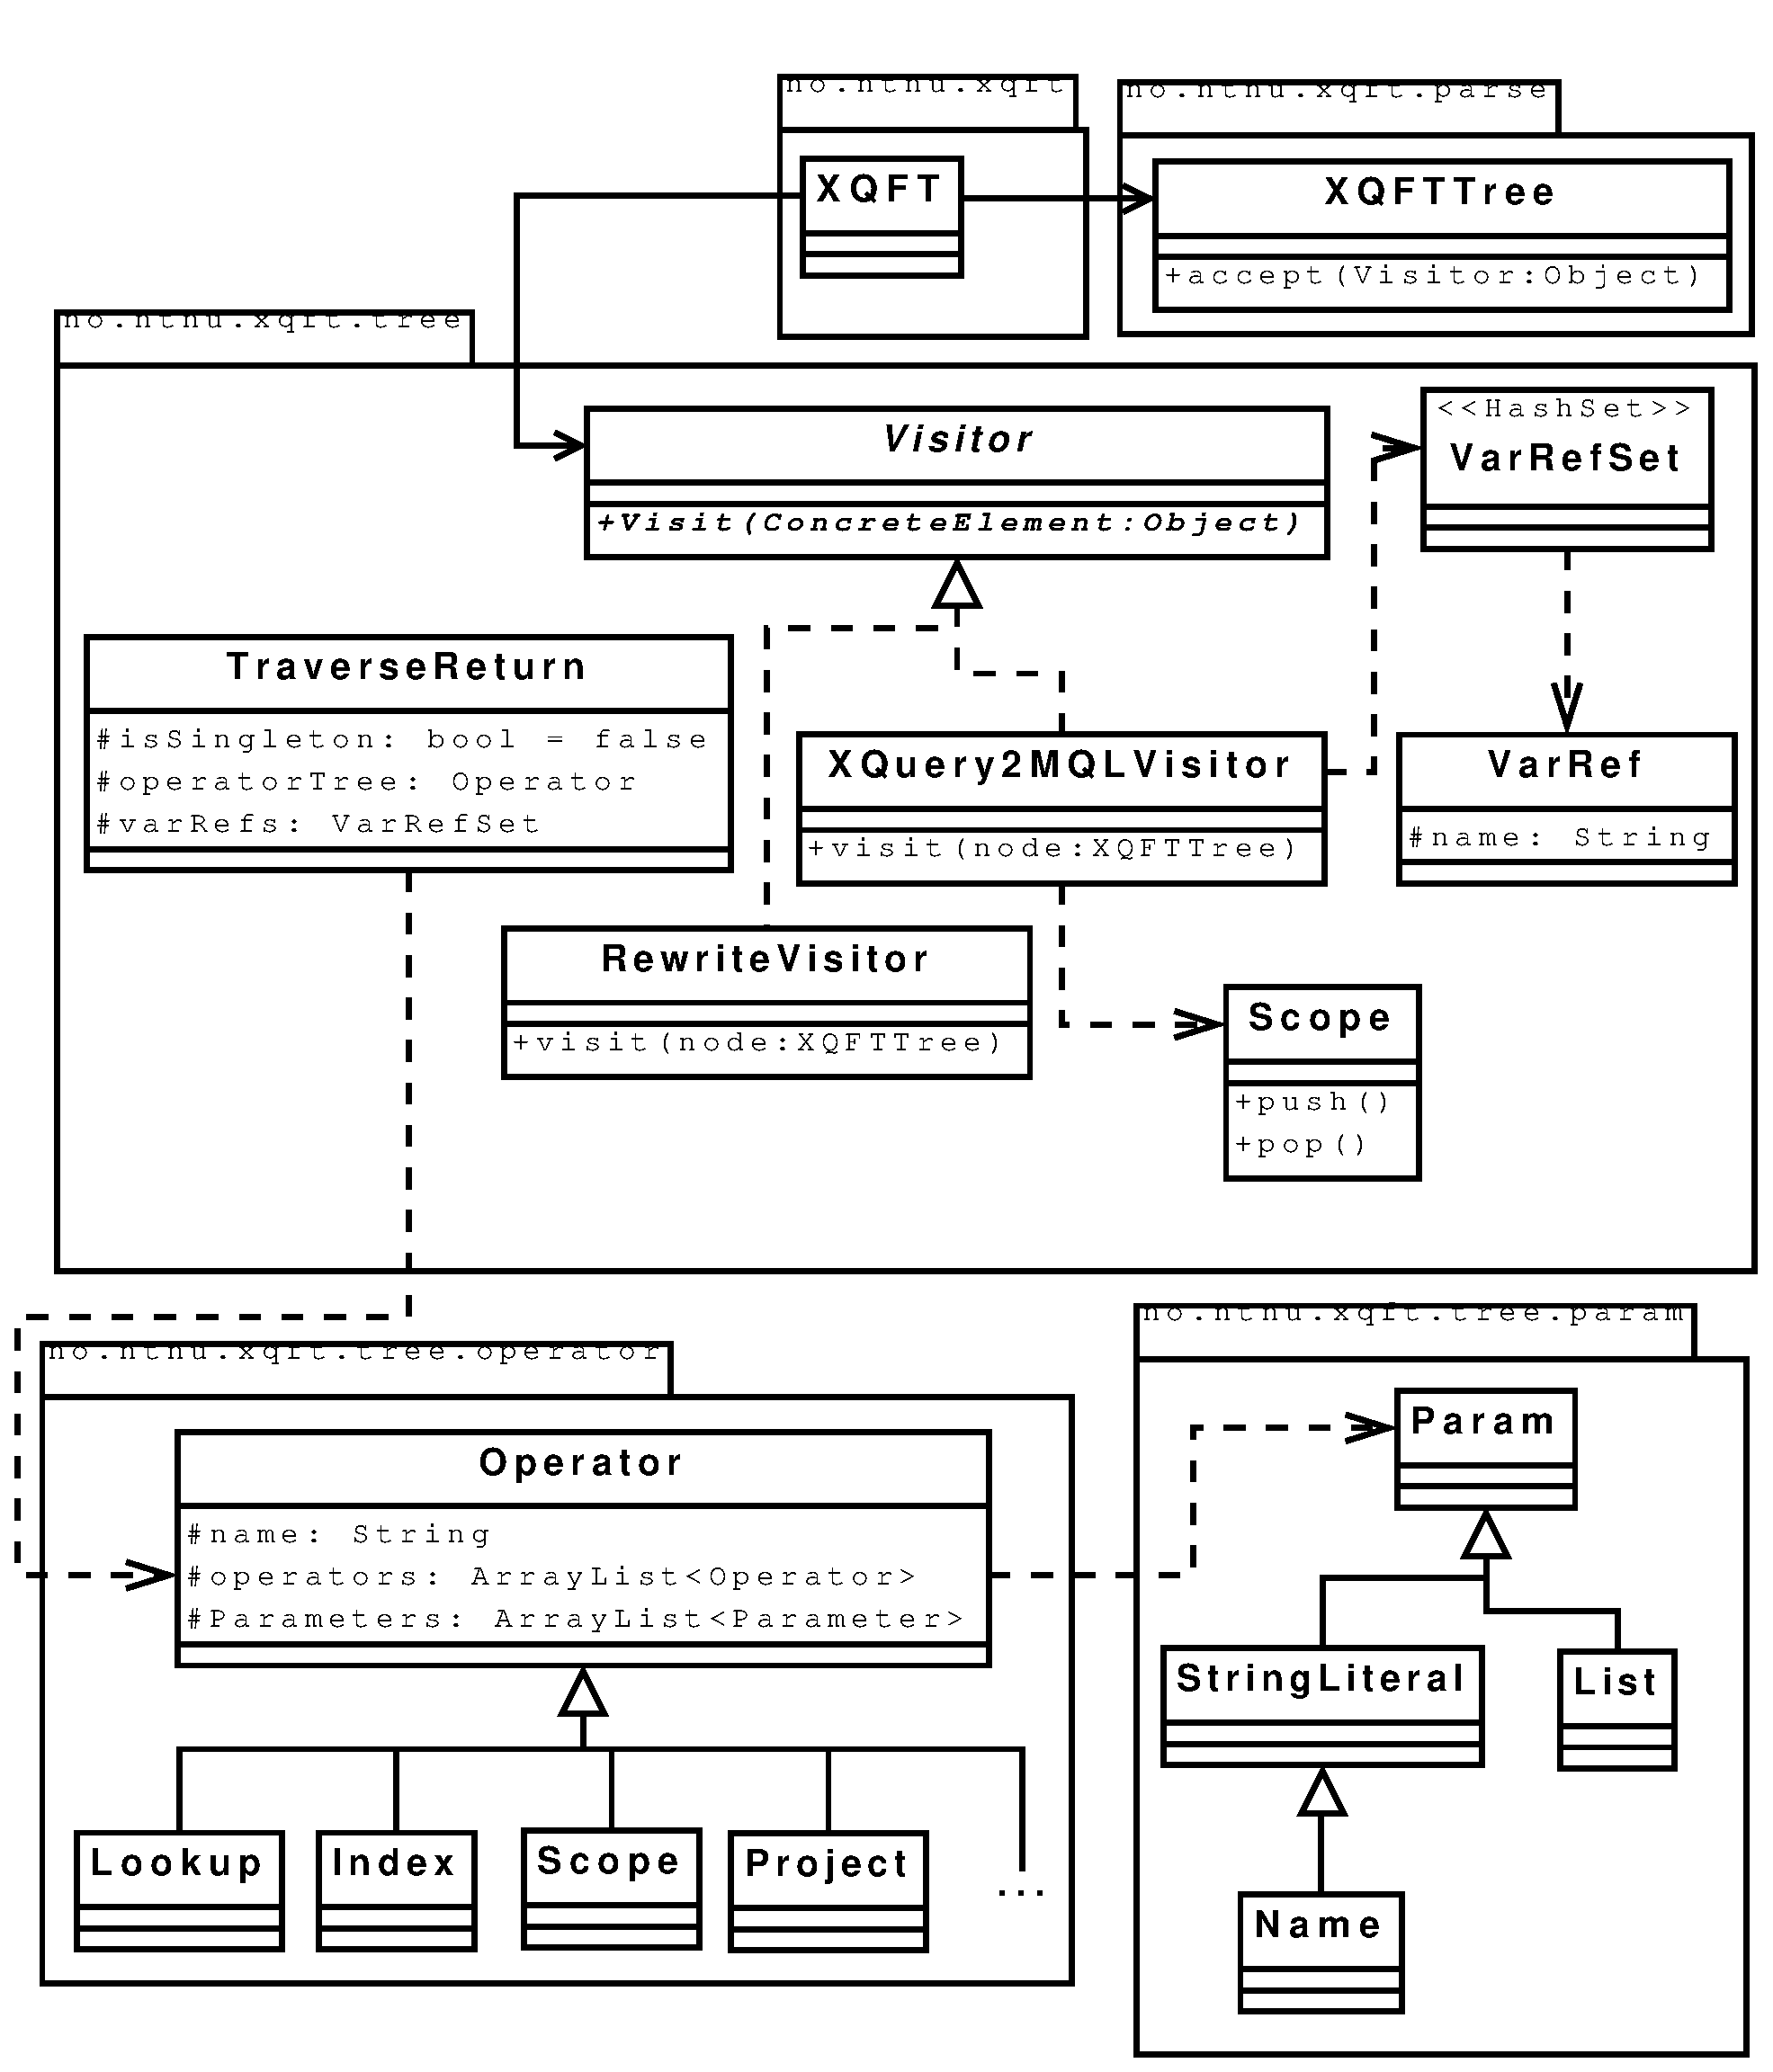
\includegraphics[scale=0.45]{diagrams/complete_uml}
  \caption{Simplified UML for complete implementation}
  \label{fig:impl:sys:uml_complete}
\end{center}
\end{figure}

\subsection{Data flow}
\begin{figure}[!htp]
\begin{center}
  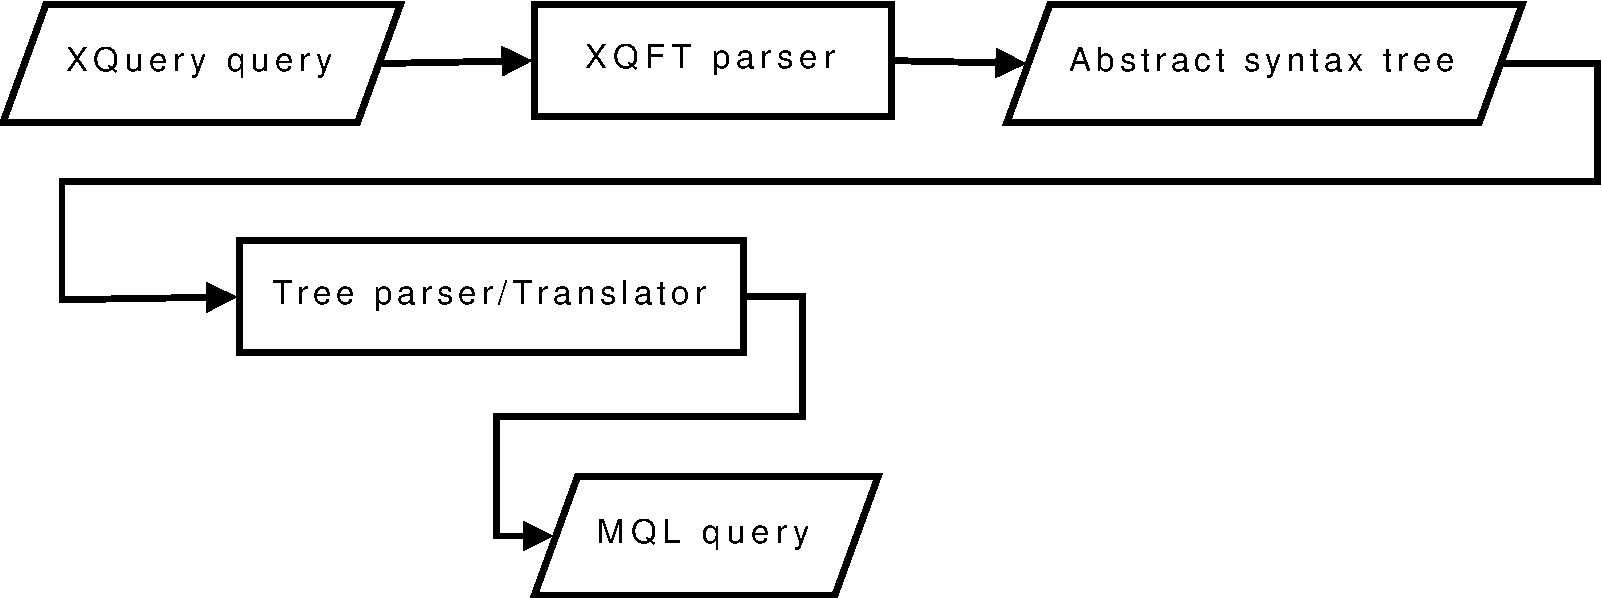
\includegraphics[scale=0.5]{diagrams/mql_dataflow}
  \caption{Data flow for XQuery parsing and translation to MQL}
  \label{fig:impl:sys:mql_dataflow}
\end{center}
\end{figure}
\subsection{Data flow}

\subsection{Visible external API}
\begin{itemize}
  \item Vise hvordan oversetteren kan brukes i sin helhet i andre programmer
\end{itemize}

\subsection{Command line interface}
\marginpar{\underline{\textbf{\Large TODO:}}\scriptsize ha det i appendix ala i fjor?}
Dette er ikke s\aa~veldig viktig \aa~skrive om, men greit \aa~ha med.
\begin{itemize}
  \item Argsengine
  \item Aksepterer flere strenger og filer
  \item Outputter til graphviz/dot og pdf, hvis tilgjengelig
  \item Dependencies (jar-filer og drit)
\end{itemize}
\section{Using the XQFT Parser}
The \textit{XQFT Parser}\cite{ourselves} (described in section
\ref{sect:theory:xqftparser}) is a prerequisite for providing the abstract
syntax tree for this XQuery translator. This section will outline how this
parser was used and interfaced with the implementation.

The \textit{XQFT Parser} is a parser generated by the ANTLR parser generator.
Thus, there is a loosely standardised API available for any implementor
utilising a parser generated by ANTLR. In the case of \textit{XQFT Parser}, two
classes are generated: \texttt{XQFTParser} and \texttt{XQFTLexer}. These
classes are used in conjunction on an input string to produce an abstract syntax
tree (see next subsection, and also section
\ref{sect:theory:xqftparser:ast_construction}).

A typical use case to achieve this is shown in figure
\ref{figure:impl:using_xqft}, which is copied almost verbatim from the
implementation.

\begin{figure}[!htp]
\begin{center}
  \begin{Verbatim}
    CharStream cs 
        = new ANTLRStringStream(
            "for $i in (1,2,3) return $i");

    XQFTLexer lexer = new XQFTLexer(cs);

    UnbufferedCommonTokenStream tokens 
        = new UnbufferedCommonTokenStream();
	tokens.setTokenSource(lexer);

    XQFTParser parser = new XQFTParser(tokens);
    parser.setTreeAdaptor(new XQFTTreeAdaptor());
    parser.setLexer(lexer);

    XQFTTree ast = parser.module().getTree();
  \end{Verbatim}
  \caption{Using the XQFTParser and XQFTLexer classes}
  \label{figure:impl:using_xqft}
\end{center}
\end{figure}
Note the use of \texttt{ANTLRStringStream},
\texttt{UnbufferedCommonTokenStream}, and \texttt{XQFTTreeAdaptor}. The latter,
\texttt{XQFTTreeAdaptor}, is a specialised class required to create instances of
the \texttt{XQFTTree} class to represent nodes in the abstract syntax tree.

The actual parsing is performed by calling the method \texttt{module()}, which
is the top-level production rule in the grammar for the XQFT parser (see
appendix \ref{appendix:xquery_ebnf}).

The \texttt{XQFTTree} class represents a node in the produced syntax tree. When
a syntax tree is returned from the parser, the root node is an instance of this
class, as well as all children (see figure \ref{figure:impl:using_xqft})

To make practical use of the XQFT Parser, what remains is nothing more than to
translate the abstract syntax tree acquired from the call to
\texttt{getTree()}, which is the object \texttt{ast} on the last line of code
in figure \ref{figure:impl:using_xqft}.

\section{Constructing the MQL algebra tree}
\label{sect:impl:construct_mql}
MQL queries are constructed as trees, where each node represents an operator. Each node is an instance of an
operator class, and may contain a list of child operators and a list of parameters. The trees are constructed
bottom-up while parsing the abstract syntax tree corresponding to a XQuery query.

\subsection{Operators and parameters}
\begin{figure}[!htp]
\begin{center}
  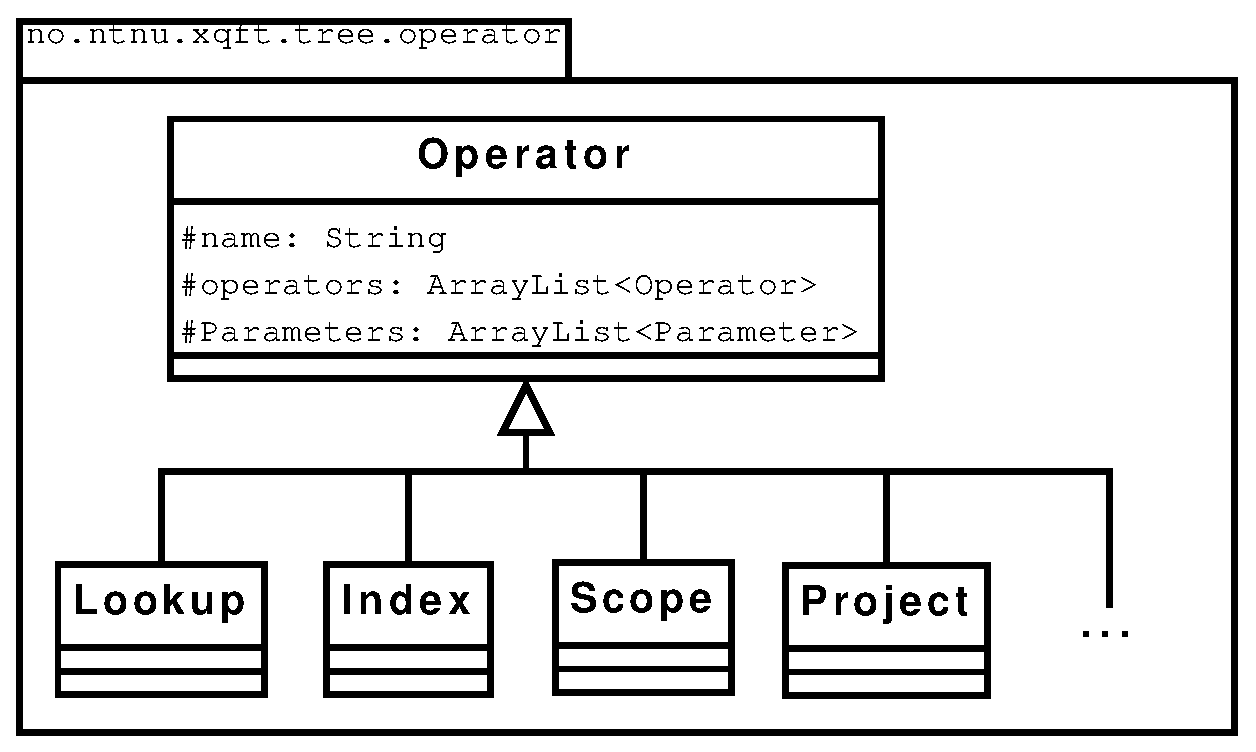
\includegraphics[scale=0.5]{diagrams/mql_operator_uml}
  \caption{Simplified class diagram of MQL operators}
  \label{fig:impl:mql_op_uml}
\end{center}
\end{figure}
The operators modeled in the implementation correspond to the operators
described in section \ref{sect:method:marsOperators}. A simplified class
diagram is shown in figure \ref{fig:impl:mql_op_uml}. Converting an operator to a string is in most cases
handled by the default fallback in the \texttt{Operator} class, where the string generated will be on the form:
\begin{Verbatim}
operator_name(param1, param2, ..., paramN; 
    operator1;
    operator2; 
    ...; 
    operatorM)
\end{Verbatim}

Constructing such a string for the complete query tree is achieved by calling \texttt{toPrettyString(0)} on the
root node. The parameter to the method specifies the initial indentation.

\begin{figure}[!htp]
\begin{center}
  \includegraphics[scale=0.5]{diagrams/mql_param_uml}
  \caption{Class diagram of MQL parameters}
  \label{fig:impl:mql_param_uml}
\end{center}
\end{figure}

MQL parameters (as described in \ref{sect:method:mql:concepts}) are modeled as
seen in figure \ref{fig:impl:mql_param_uml}. Parameters require no complex
structure, and are only created and added to operators as needed.

\subsection{Usage}
The operator classes are designed to be intuitive and simple to use. Figure
\ref{fig:impl:mql_op_ex1_java} shows one example where a simple operator tree
is built and converted to an MQL query string. The result can be seen in figure \ref{fig:impl:mql_op_ex1_mql}).

%\usepackage{graphics} is needed for \includegraphics
\begin{figure}[htp]
\begin{center}
  \begin{Verbatim}
Lookup lookup = new Lookup("Death in the clouds");
Scope scope = new Scope("/books/book/title", lookup);
Project project = new Project("author", scope);
System.out.println(project.toPrettyString(0));
  \end{Verbatim}
  \caption{Example java code to construct a MQL operator tree}
  \label{fig:impl:mql_op_ex1_java}
\end{center}
\end{figure}

\begin{figure}[htp]
\begin{center}
  \begin{Verbatim}
project(author;
  scope(/books/book/title;
    lookup("Death in the clouds")))
  \end{Verbatim}
  \caption{Resulting MQL query string from example in figure
  \ref{fig:impl:mql_op_ex1_java}}
  \label{fig:impl:mql_op_ex1_mql}
\end{center}
\end{figure}

\section{Context-sensitive visitor}
In section \ref{sect:theory:parser:tree_parsing} a number of techniques for
tree parsing were presented. In section \ref{sect:method:tree_parsing} the
\textit{context-sensitive visitor pattern} was chosen as the technique for this
implementation. This section will detail the implementation of this design
pattern, and how it is used to performed an assortment of tasks.

\subsection{Basics}
The context-sensitive pattern is designed to be flexible and to generate code
with a higher level of maintainability, for which the rationale was presented
in section \ref{sect:theory:contextVisitorPattern}. 

\begin{figure}[htp]
\begin{center}
  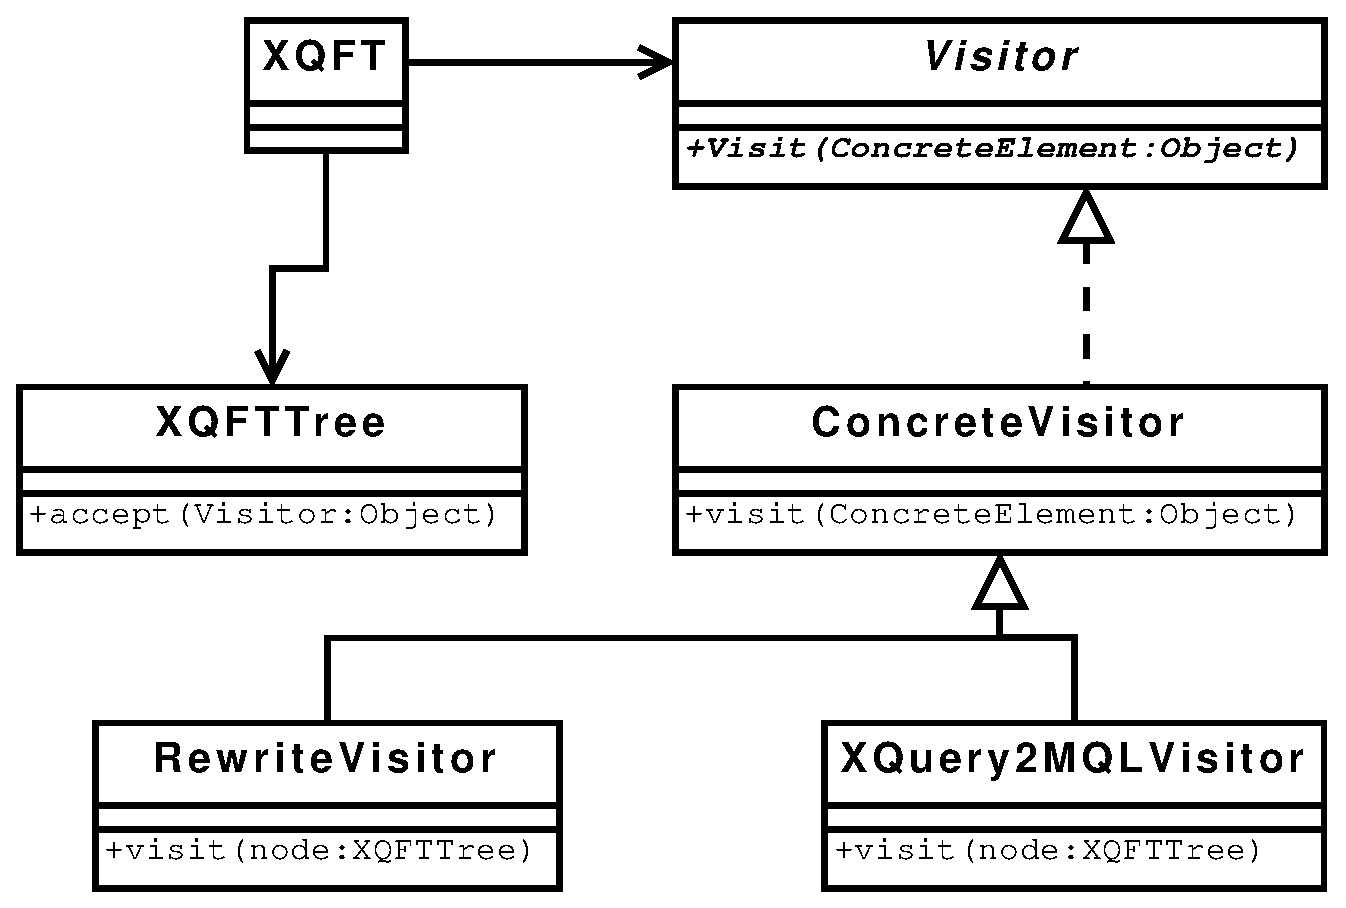
\includegraphics[scale=0.5]{diagrams/context_visitor_pattern_impl}
  \caption{Context sensitive visitor implementation}
  \label{fig:impl:context_sens_visitor_impl}
\end{center}
\end{figure}

The class diagram for the actual implementation of the context-sensitive
visitor pattern can be seen in figure \ref{fig:impl:context_sens_visitor_impl}.
Compare this to the generalized class diagram in figure
\ref{figure:parser:context_visitor_pattern} on page
\pageref{figure:parser:context_visitor_pattern}.

Note that the use of \texttt{XQFTTree} as the element class implies that the
\texttt{XQFTTree} be supplemented with an \texttt{accept()} method to
accommodate this pattern. This method is essentially a static dispatcher which
will call the appropriate method on the visitor based on the token type of the
node currently being visited. Figure \ref{} shows an excerpt of this method and
how it acts on the visitor class.

%\usepackage{graphics} is needed for \includegraphics
\begin{figure}[htp]
\begin{center}
  \begin{Verbatim}	
public TraverseReturn accept(Visitor visitor) {
     case XQFTParser.AST_MODULE:
            return visitor.visitAST_MODULE(this);
        case XQFTParser.AST_FLWOR:
            return visitor.visitAST_FLWOR(this);
        case XQFTParser.AST_FORCLAUSE:
            return visitor.visitAST_FORCLAUSE(this);
        case XQFTParser.AST_LETCLAUSE:
            return visitor.visitAST_LETCLAUSE(this);
        case XQFTParser.AST_ORDERBYCLAUSE:
            return visitor.visitAST_ORDERBYCLAUSE(this);
        case XQFTParser.AST_WHERECLAUSE:
            return visitor.visitAST_WHERECLAUSE(this);
                          .
                          .
                          .
  \end{Verbatim}
  \caption{Excerpt from the accept() method in the XQFT class}
  \label{figureLabel}
\end{center}
\end{figure}

\subsection{The Rewrite visitor}
The \textit{Rewrite visitor} is used to perform rewrite operations on the
abstract syntax tree before performing the actual translation. In particular,
these rewrite operations consists of normalizing the required subtrees of the
syntax tree to a subset of XQuery Core.

\subsection{The Translation visitor}
\section{Scoping and symbol tables}
Crucial to the implementation of the \textit{tainting dependencies} methodology
described in section \ref{sect:trans:taintingDependencies} is the ability to
maintain a contextual environment with scoping and symbol tables. This section
details the implementation of this, and how it is used to achieve the
requirements of \textit{tainting dependencies}.

\subsection{Concepts}
The scoping system in the implementation is based on building a scope tree. The
previous scope, if any, is set as parent of the new scope, and the previous
scope maintains a list of child scopes. A reference to the root scope node is
maintained. Considering the example XQuery query in figure
\ref{fig:impl:scope_tree_ex_code}, the scope tree in figure
\ref{fig:impl:scope_tree_ex} is generated.

\begin{figure}[!htp]
\begin{center}
\begin{Verbatim}
for $i in (1,2,3) return 
  for $a in (4,5,for $b in (6,7,8) return $b) 
    return ($i,$a)
\end{Verbatim}
  \caption{Scope tree example code}
  \label{fig:impl:scope_tree_ex_code}
\end{center}
\end{figure}


\begin{figure}[!htp]
\begin{center}
  %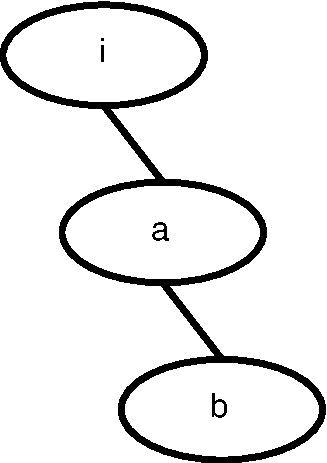
\includegraphics[scale=0.5]{diagrams/scope_tree_ex}
  \textbf{\Large TODO} bildet mangler
  \caption{Scope tree for source code in figure
  \ref{fig:impl:scope_tree_ex_code}}
  \label{fig:impl:scope_tree_ex}
\end{center}
\end{figure}

Entries in the symbol table are represented through an instance of the
\texttt{SymTabEntry} class which maintains metadata about symbols (such as
symbol name, a flag indicating whether it's an iterator variable, and an
evaluated expression). The symbol table is realized as a subclass of the
\texttt{HashMap} class in the \texttt{java.util} package, and is constrained to
storing instances of \texttt{SymTabEntry}, with the symbol name as key.

\subsection{Semantics}
The scoping semantics is encapsulated in a singleton manner in the class
\texttt{Scope}, with static methods available for pushing and popping scopes,
and storing and retrieving symbols. The external (static) API as available to a
user of the scope system is shown in figure \ref{fig:impl:scope_uml}.

\begin{figure}[!htp]
\begin{center}
  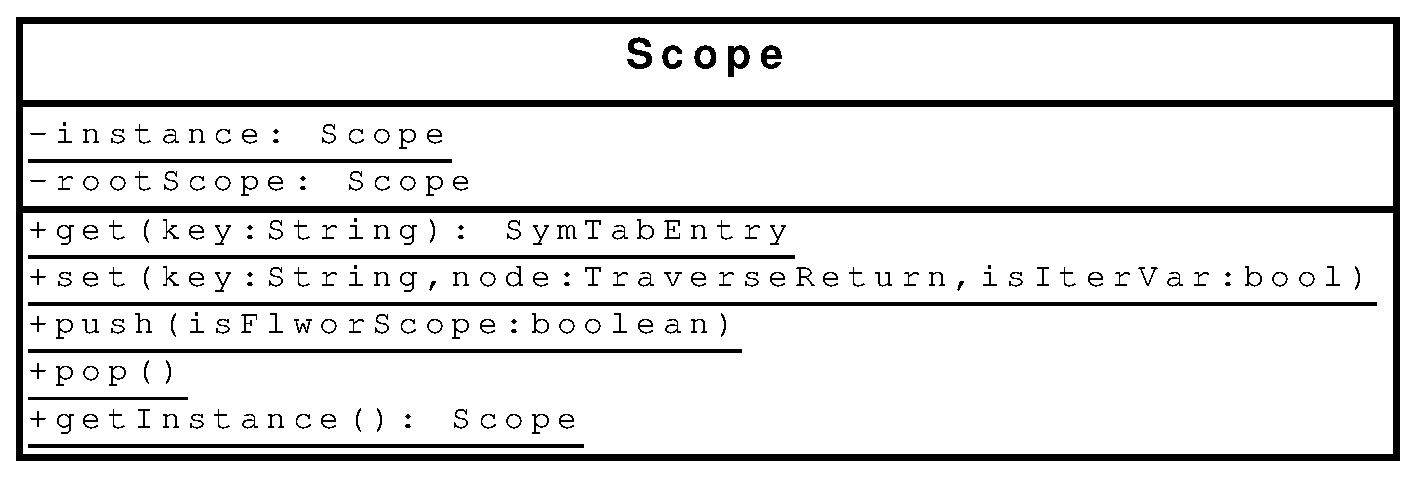
\includegraphics[scale=0.5]{diagrams/scope_uml}
  \caption{Scope API}
  \label{fig:impl:scope_uml}
\end{center}
\end{figure}

A new scope is \textit{pushed} whenever a for-clause is encountered while
parsing the abstract syntax tree, and the current scope is \textit{popped} while
evaluating a return clause -- both of which occur within a FLWOR expression.

The scoping system also tracks iteration variables. That is, for any scope,
there is \textit{one and only one} iteration variable, except in the top scope
where there is no iteration variable. The concept of an iteration variable is
explain in definition \ref{} TODO: definisjon av iteratorvars. Tracking these
variables are necessary to implement the \textit{tainting dependencies} methodology (explained
later in section \ref{sect:impl:tainting_deps} on page
\pageref{sect:impl:tainting_deps}).
\section{Passing metadata between nodes}
\subsection{Variable references}
\subsection{Singleton nodes}
\subsection{The TraverseReturn class}
\section{Tainting dependencies}
\label{sect:impl:tainting_deps}
``Tainting dependencies'' is a method of translating XQuery queries to
relational algebra. The semantics of this method is described in detail
throughout section \ref{sect:trans:taintingDependencies}. This section
describes an implementation of a subset of this method which is capable of
translating simple FLWOR expressions, sequences, and variables. 

\subsection{FLWOR expressions}
The translation process for FLWOR expressions were outlined in section
\ref{sect:trans:TD:simpleFLWOR}. Consider inference rule
\ref{rule:trans:TD:forbind} on page \pageref{rule:trans:TD:forbind}. This
inference rule states how to translate and bind an iterator variable in a
for-clause in a FLWOR expressions. The implementation of this inference rule is
shown in figure \ref{fig:impl:td:varbindfor}. This excerpt includes two visitor
methods. First a for-clause is visited, and the child is flagged as a FLWOR
tuplet definition (lines 1 through 7). Next a dollar sign is visited (which
carries the meaning of a variable in the abstract syntax tree). If the child
count is more than one, it is an assignment. Note that the
\texttt{isIterationVar} flag is \textit{true} if this assignment is a tuple
definition as flagged earlier.

Then, if this is an assignment and a tupled definition, the right-hand side of
the assignment is translated, and the symbol is entered into a symbol table.
Note that the creation of the project operator is required by inference rule
\ref{rule:trans:TD:forbind}.

This example can be better understood if seen in context of an abstract syntax
tree example. Considering the example in figure \ref{fig:impl:td:flwor2}. Here
the \textit{AST\_FORCLAUSE} node will be visited by the
\texttt{visitAST\_FORCLAUSE()} method in the visitor and the
\texttt{isFlworTupleDef} flag will be set to \textit{true}. Then the variable
node (the dollar sign) will be visited by the \textit{visitDOLLARSi()} method,
and the translation of the for clause is completed.

\begin{figure}[!htp]
\begin{center}
\lstset{language=Java,numbers=left}
\begin{lstlisting}
    public TraverseReturn visitAST_FORCLAUSE(XQFTTree tree) {
        
        ((XQFTTree)tree.getChild(0)).setFlworTupleDef(true);
        acceptThis(tree.getChild(0));

        return null;
    }
    .
    .
    .
    
    public TraverseReturn visitDOLLARSi(XQFTTree tree) {
        
        boolean isIterationVar = tree.isFlworTupleDef();
        
        String varName = tree.getChild(0).getText();
        
        // Assignment?
        if (tree.getChildCount() > 1) {
            
            // Visit children on the right side of the assignment
            TraverseReturn tr = acceptThis(tree.getChild(1));
            
            // Required for tainting deps method
            Project project = new Project(
                "[" + varName + "numb, value]", 
                tr.getOperatorTree());

            // Assign metadata
            tr.setOperatorTree(project);
            tr.setSingleton(true);
            
            // Enter into symbol table
            SymTabEntry tmp = Scope.set(tree.getChild(0).getText(), 
                                  tr, isIterationVar);
            
            if (isIterationVar) {
               Scope.getInstance().setCurrentIterVar(
                                       new VarRef(tmp.getName()));
            }
            
            return tr;
        }
        .
        .
        .
\end{lstlisting}
  \caption{Translation and binding of iteration variables}
  \label{fig:impl:td:varbindfor}
\end{center}
\end{figure}

%\usepackage{graphics} is needed for \includegraphics
\begin{figure}[!htp]
\begin{center}
  \includegraphics[scale=0.4]{img/graphs/flwor2}
  \caption{FLWOR syntax tree example}
  \label{fig:impl:td:flwor2}
\end{center}
\end{figure}

Following the translation of the for-clause, the return clause is translated in
a similar manner. However this translation is slightly more complicated. The
translation is dependent on whether the return clause contains code which
references the current iteration variable. If this is the case, then a
translation which applies tainting given by the rule in figure
\ref{eq:trans:TD:taint} page \pageref{eq:trans:TD:taint} must be used. In
particular, the rule in figure \ref{rule:trans:TD:returnTaint} shown on page
\pageref{rule:trans:TD:returnTaint} must be applied (which implies the former).

\begin{figure}[!htp]
\begin{center}
\lstset{language=Java,numbers=left}
\begin{lstlisting}
// Sort and partition fields
String[] sortBy = {Scope.getInstance().getCurrentIterVar().getName() 
		          + "numb", "index"};
String[] partitionBy 
	= new String[returnClauseResult.getVarRefs().size() - 1];

// Calculate variable references
VarRefSet prevVarRefs 
	= (VarRefSet)returnClauseResult.getVarRefs().clone();         
prevVarRefs.remove(Scope.getInstance().getCurrentIterVar());

int i = 0;
for (VarRef ref : prevVarRefs) {
    partitionBy[i] = ref.getName();
    i++;
}

// Construct MQL
Numberate numberate = new Numberate("index", 
                                    sortBy, 
                                    partitionBy, 
                                    returnClauseResult.getOperatorTree());

// Construct result
TraverseReturn result = new TraverseReturn();
result.setSingleton(false);
result.setVarRefs(returnClauseResult.getVarRefs());
result.setOperatorTree(numberate);

// Remove current iter var from varrefs
result.getVarRefs().remove(Scope.getInstance().getCurrentIterVar());

Scope.pop();
return result;
\end{lstlisting}
  \caption{Translation of a return clause with a reference to the current
  iteration variable}
  \label{fig:impl:td:for_return_withref}
\end{center}
\end{figure}

Figure \ref{fig:impl:td:for_return_withref} shows how this has been
implemented. Note that the code in this example is executed if and only if
there is a reference to the iteration variable in the return clause.

If there is no reference to the current iteration variable, then the
translation is done as usual per rule 

\subsection{Sequences}
\label{sect:impl:td:seq}
The translation process for sequence construction is described in section
\ref{sect:trans:TD:seqBuild}. This rule is somewhat complex, and requires
collecting all variable references from all children before performing the
actual translation. Furthermore, for any variable reference in a left-most
child, this variable reference must taint all right-most children. This process
is shown in figure \ref{fig:impl:td:seq_constr_tainting_siblings}.

\begin{figure}[!htp]
\begin{center}
\lstset{language=Java,numbers=left}
\begin{lstlisting}
for (TraverseReturn childResult : childResults) {
    VarRefSet varRefsDiff;
    Operator expr = childResult.getOperatorTree();
    
    VarRefSet tmp = childResult.getVarRefs();
    varRefsDiff = (VarRefSet)varRefs.clone();
    varRefsDiff.removeAll(tmp);

    for (VarRef varRef : varRefsDiff) {
        Project project = new Project(varRef.getName() + "numb", 
                Scope.get(varRef.getName()).getTraverseReturn().getOperatorTree());
        
        Cross cross = new Cross(project, expr);
        expr = cross;
    }

    if (childResult.isSingleton()) {
        expr = new Project("sprIdx="+(c+1)+",index,value", expr);
    }
    else {
        expr = new Project("sprIdx="+(c+1)+",value", expr);
    }
    operators.add(expr);
    c++;
}
\end{lstlisting}
  \caption{Tainting siblings in a sequence construction}
  \label{fig:impl:td:seq_constr_tainting_siblings}
\end{center}
\end{figure}

This will propagate tainting throughout the siblings as required. When this
procedure is complete, the operator tree in the \texttt{operators} variable is
wrapped in a \textsf{union()} operator. Etc.

\begin{itemize}
  \item behandler parantes istf. komma for sekvenser (ref spec) 
\end{itemize}

\subsection{If-then-else}
TODO: Skrive om if-then-else? comparisons??






\section{Optimalisations?}

\section{Summary}
\label{sect:impl:summary}
\begin{itemize}
  \item sammendrag av dette kap
\end{itemize}